\documentclass[11pt,a4paper]{article}

\usepackage[margin=2cm]{geometry}
\usepackage[utf8]{inputenc}
\usepackage[english]{babel}
\usepackage{amsmath}
\usepackage{amsfonts}
\usepackage{amssymb}
\usepackage{graphicx}
\usepackage{hyperref}

%added userpackages
\usepackage{microtype}
\usepackage{natbib}
\usepackage{lmodern}
\usepackage{bmpsize-base}
\usepackage{xcolor}




%%%%%%%%%%%%%%%%%%%%%%%%%

\title{Graph-Based Analysis of Gene Activity in Lung Cancer based on Protein-Interaction Networks}
\author{
Simone Bergmann, 3957624 \\
\texttt{simone.bergmann@uni-bielefeld.de}%
}
%%%%%%%%%%%%%%%%%%%%%%%%%
% \twocolumn
\begin{document}
\maketitle

% FACTS:
% 15 bis 30 Seiten (exklusive Titel, Abstract, Inhaltsverzeichnis, Literaturverzeichnis, ...)
% Deckblatt
% Inhaltsverzeichnis
% Nicht zu viele Unterkapitel / zu sehr verschachtelt
% ca 30 Quellen
% Jedes Kapitel am Anfang und am Ende zusammenfassen aber Fokus auf Ende



{\color{lightgray}
Task:
Creation of a data model and integration of genes and proteins with interactions in an appropriate form within a graph database,
which is to be used for the identification of relevant genes for distinguishing between healthy tissue and lung cancer.

Key facts:
* cancerous mean tpm from Cell Model Passport \\
* healthy mean tpm from Genotype-Tissue Expression \\
* delta tpm as difference between healthy and cancerous tpm \\
* genes are connected with proteins and proteins are connected with each other (STRING database) \\
* neo4J as graph database \\
* pagerank as graph algorithm to identify relevant genes \\
}

% TODO
% Abstact soll kursiv sein

\begin{abstract} \label{abstract}

    Lung cancer remains one of the leading causes of mortality worldwide,
    with significant implications for public health and individual well-being.
    To address this challenge,
    we aim to contribute to the ongoing efforts to combat lung cancer by identifying potential biomarkers using graph databases and algorithms.
    Traditional methods often struggle to capture the complex relationships between genes and proteins.
    We try to overcome these challenges with a graph based approach.
    By analyzing gene expression data and applying a network-based approach,
    we have successfully identified 10 genes that may serve as biomarkers for early detection or personalized treatment.
    Our method integrates over 17,000 genes, 100,000 proteins, and 13,000,000 interactions,
    allowing us to pinpoint relevant genes with high connectivity in the network.
    This approach has revealed promising new targets for further research and
    underscore the importance of considering gene interactions in cancer development.
    While our study provides valuable insights into the genetic landscape of lung cancer,
    it is essential to note that further validation and refinement of our methodology are necessary to ensure the accuracy and reliability of our findings.

\end{abstract}

\section{Introduction} \label{sec:intro}


% TODO könnte noch etwas länger sein
\subsection{Motivation} \label{subsec:motivation}
% 300 Words

% Problem
Lung cancer is a major public health problem worldwide, caused by various factors,
including smoking, air pollution, and also genetic factors.
It is the leading cause of cancer-related deaths worldwide\cite{ferlay2024global}.
Despite advances in medical care, the survival rate for patients remains relatively low,
with only $30.2\%$ of women and $22.1\%$ of men (2016)
surviving beyond five years after diagnosis~\cite{seer2024explorer}, often due to late-stage detection.
Early detection is therefore crucial to initiate timely treatment and ultimately reduce the mortality rate.

% Solution
We focus on analyzing gene expression data to identify potential biomarkers for lung cancer.
We use graph databases for this purpose,
as they offer ways to represent complex relationships between large sets of genes and proteins
and analyze them efficiently using algorithms.
These data provide valuable insights into the underlying molecular mechanisms of lung cancer
and thus help to improve the early diagnosis and treatment of lung cancer.

\subsection{Goals} \label{subsec:goals}
The main goal of this thesis is to identify potential biomarkers for lung cancer by examining gene activity data.
These Biomarkers could be used for early detection or personalized treatment.
This will be done by uncovering genes with altered cancer activity that are closely connected to other genes.

To achieve this goal, we have three strategic objectives:
\begin{enumerate}
    \item \textbf{Objective - Find significant changes in gene activity:}\\
    We must first decide on an appropriate measurement for cancer-related changes in gene activity.
    Next, we will compare this gene activity measure for healthy and cancerous tissues to identify genes with substantial differences.
    These genes will serve as our focus for further analysis.
    \label{obj:delta_tpm}

    \item \textbf{Objective - Application of a graph algorithm:}\\
    We will construct a graph database containing genetic information with connections between genes and proteins.
    By applying a graph algorithm, we aim to identify the most central genes in the network,
    which may have the highest impact on other genes.
    \label{obj:graph_algorithm}

    \item \textbf{Objective - Validation of results through study comparison:}\\
    We will assess the relevance and novelty of our findings by comparing them with existing research on lung cancer.
    By validating our results against established knowledge, we want to ensure that our identified genes are potential biomarkers.
    \label{obj:validation}
\end{enumerate}

These objectives provide a roadmap for achieving our main goal.
By determining significant changes in gene activity, applying graph algorithms,
and validating results through comparisons with existing research,
we aim to contribute meaningfully to lung cancer research.


% TODO zum Schluss wenn ich weiß was genau wo drin ist
\subsection{Structure}  \label{subsec:structure}

{\color{lightgray}

The chapter \ref{sec:background}provides a detailed overview of the biological and computational background of the project,
including facts about lung cancer, the importance of gene expression analysis and the use of graph databases in cancer research.

In the third chapter \ref{sec:experimental-setup}, we will describe the setup,
including the data sources and the creation of the graph database.

The fourth chapter \ref{sec:results} presents the results of the graph analysis and the identified relevant genes.

The fifth chapter \ref{sec:discussion} discusses the results and compares them with other studies.

The final chapter \ref{sec:conclusion} summarizes the findings and provides an outlook on future research.

}

\subsection{Limitations} \label{subsec:limitations}

{\color{lightgray}
Our Analysis has the following limitations:
\begin{itemize}
    \item The data used in this project is limited on human genes.
    \item We focussed on the analysis of lung cancer.
    \item The gene expression data used in this project is limited to TPM values from the GTEx and Cell Model Passport datasets.
\end{itemize}

% nur auf protein codierende Gene beschränkt
}



\section{Background} \label{sec:background}
In this chapter we will take a closer look at the biological and computational background of our project.
Also, we will discuss related work in the field cancer research with graph databases.

\subsection{Biological background} \label{subsec:biological_background}
To have a better understanding of our project, we need to have a closer look at some biological topics and concepts.

% Cancer overview
\textbf{Cancer} is a complex, multifactorial disease characterized by uncontrolled cell growth.
Research shows that widespread metastases are the primary cause of death from cancer~\cite{who_cancer_fact_sheet}
and that cancer comes in more than 100 different types~\cite{nci_cancer_types}.

The five most common forms of cancer worldwide in 2022 were lung cancer ($>2.4$ million),
breast cancer ($>2.2$ million), colorectal cancer ($>1.9$ million), prostate cancer ($>1.4$ million) and
stomach cancer ($>0.9$ million).
In 2022, cancer was one of the leading causes of death globally,
with approximately 10 million fatalities~\cite{ferlay2024global}.

It can be caused by a combination of genetic and environmental factors,
such as diet, radiation, age, exposure to certain chemicals or viruses~\cite{nci_cancer_risk}.
Early detection and the right treatment can significantly improve the chances of curing many types of cancer.
\\

% lung cancer
In this study we will focus on \textbf{Lung cancer}, a type of cancer that affects the lung organ.
There are two subtypes: non-small cell carcinoma (NSCLC) and small cell carcinoma (SCLC)~\cite{nci_lung_cancer_types}.
The primary risk factor for developing lung cancer is smoking,
but passive smoking and environmental pollution also significantly increase the risk~\cite{nci_lung_cancer_types}.

Symptoms of lung cancer often resemble those of common colds or other minor illnesses, such as coughing and fatigue.
This makes it challenging for patients to receive timely treatment, often leading to a diagnosis at an advanced stage~\cite{who_lung_cancer}.
\\

% gene expression
\textbf{Gene expression} is a crucial factor in the investigation of cancer.
It describes the process of transcribing DNA into RNA molecules that code for proteins,
which are then translated and regulated through complex interactions to control the production
and function of gene products~\cite{nhi_gene_expression}.
Alterations in gene expression can contribute to the uncontrolled multiplication and abnormal behavior of cancer cells,
which ultimately leads to the development and progression of cancer~\cite{ferlier2022regulation}.
\\

%TPM
To accurately compare gene expression data across different experiments, it is essential to normalize and quantify the expression levels.
The most commonly used metrics for this purpose include Reads per million mapped reads (RPM),
Reads Per Kilobase Million (RPKM), Fragments Per Kilobase Million (FPKM),
and Transcripts Per Kilobase Million (TPM)~\cite{cd_geneomics_gene_expression}.
Among these measures, \textbf{TPM} is widely adopted in available datasets.
Therefore, we will utilize it as our metric of choice for quantifying gene expression levels.
\\

% Gene IDs
A common way to identify genes is through the use of unique identifiers known as \textbf{ENSEMBLE IDs}.
These are unique ids for genes, proteins and other genetic elements collected in the Ensemble database
from 1999 by the European Bioinformatics Institute and the Wellcome Trust Sanger Institute~\cite{ensembl_project}.
These make it easier to compare and analyze gene data across different datasets.
\\

% Multiomics data
Omics is a collection of fields in biology that end in -omics, such as genomics, proteomics, metabolomics, etc.~\cite{subedi2022omics}.
\textbf{Multi-omics data}, the combination of data from different omics fields,
are used to gain a better understanding of associations between biological molecules (e.g., genes and proteins) and their interactions
~\cite{Subramanian2020MultiomicsDI}.
Since we will be using genes and proteins in our study, we also have a multi-omics approach.
\\

\subsection{Computational background} \label{subsec:computational_background}
% TODO - K - noch mehr Quellen?

% Graph databases
\textbf{Graph databases} are an effective way to model and analyze graph-like data,
which is in contrast to traditional relational databases well-suited for applications involving relationships between entities.
For instance, social networks and biological systems can be effectively represented using these graph structures~\cite{graph_db_survey}.
In particular, graph databases have been widely used in biological data analysis, such as modeling Protein-Protein-Interaction (PPI) networks
that illustrate the interaction between proteins to control cellular processes.
In this thesis, we use a graph database to put our collected cancer data into a meaningful context.

Just like a graph, a graph database consists of two basic components: nodes and edges between nodes.
These components form the foundation for storing and analyzing large amounts of data.

Nodes are the units that store the basic information of a certain type of entity~\cite{graph_db_survey}.
In our case, genes and proteins are represented as two different node types in the database.
Each gene is, therefore, a node with properties, such as an $ID$, a $name$ or a $TPM value$ for its activity.

Relationships between two nodes are represented by an edge, which also can be of different types.
In our graph database, for example, there are “interactions” as edges between proteins and “connections” as edges between a gene and a protein.
As in common graph theory, edges can represent structures like one-to-many or many-to-many relationships.
Edges can also have weights, directions, or properties like $name$ or $type$\cite{graph_db_power_limitations}.
We do not use these additional metadata in our setup, but they could be used to model more complex relationships.

We will implement our graph database using Neo4J, since it is a widely used graph database management system.
% TODO - K - okay so?
\\


% TODO - K - Another Sentence?
\textbf{Graph database algorithms} enable the efficient analysis and extraction of meaningful insights from large-scale network data.
They can be broadly categorized into three primary groups, which provide different perspectives on graph structure.

Traversal and Pathfinding Algorithms enable the identification of shortest or
most optimal paths between nodes in the graph, thereby facilitating the exploration of network topology.
Examples include Depth-First-Search, Breadth-First-Search, Shortest Path, and Max-Flow-Min-Cut\cite{neo4j_graph_algorithms}.

Centrality Algorithms are instrumental in understanding which nodes within a graph hold significant importance.
By evaluating centrality measures such as degree centrality, closeness centrality, betweenness centrality,
and PageRank, valuable insights into the underlying network structure is gained\cite{neo4j_graph_algorithms}.

Community Detection Algorithms, also known as clustering or partitioning algorithms,
are essential for identifying groups of nodes within a graph that share similar characteristics
or exhibit extensive connectivity.
Examples include Label Propagation, Louvain Modularity, and Strongly Connected Components~\cite{neo4j_graph_algorithms}.
\\


% PageRank algorithm
In our analysis, we utilize the \textbf{PageRank algorithm} to identify influential nodes within the network
based on their connectivity and centrality.
The PageRank algorithm was originally a method for evaluating and prioritizing websites on the internet.
It was developed by Larry Page and Sergey Brin in 1988 at Stanford University ~\cite{page1999pagerank},
the founders of Google.
The general idea behind the algorithm was that the more links pointing to a website, the more important it is.
This concept is extended in the PageRank algorithm, which assigns a node's score by iteratively considering not only its direct connections
but also the indirect relationships through its linked neighbors.

The algorithm calculates a PageRank score per node using the following formula:

\begin{align*}
PR(A)=(1-d)+d(\frac{PR(T_1)}{C(T_1)}+\dots+\frac{PR(T_n)}{C(T_n)})
\end{align*}

where $PR(A)$ is the PageRank score of node $A$,
$T_1$ to $T_n$ are nodes with edges to $A$,
$d$ is the damping factor,
and $C(T_1)$ represents the number of edges to node $T_1$~\cite{neo4j_graph_algorithms}.


% TODO - K - needed?
%This allows us to identify key regulatory genes.
%By leveraging Neo4J's graph database capabilities,
%we can efficiently compute PageRank scores for our gene activity network,
%providing valuable insights into the complex relationships between genes.



\subsection{Related work} \label{subsec:related_work}
    % related work
        % Similar projects that use graph databases for biological data analysis
        % Advantages and disadvantages of using graph databases for biological data analysis
        % How this project differs from other projects that use graph databases for biological data analysis


Overall, in the course of this background section,
we have gained a comprehensive overview of the biological background of lung cancer and
the importance of gene expression analysis.
In particular, we have looked at TPM values, which are an important measure of gene activity.

We have established that the use of graph databases is an effective way to analyze complex networks,
and we have explained corresponding algorithms, especially the PageRank algorithm.

Finally, we have reviewed related work in the field of graph databases in cancer research.


\section{Experimental Setup} \label{sec:experimental-setup}
% → rename Methodology or Implementation
\subsection{Data} \label{subsec:data}

\subsection{Methodology} \label{subsec:methodology}




\section{Results} \label{sec:results}
% focus on the results, not on the analysis

% intro
Within this chapter, we present the crucial component of our study,
where we distill the essence of the extended PPI network by identifying the top 10 genes that stand out as significant contributors.
These genes have been selected based on their high connectivity and substantial change in gene activity within the network.\\

% General Result of the PageRank
Before exploring these key genes,
it is essential to provide an overview of the distribution of PageRank scores and $\Delta_{TPM}$ values across the gene dataset.
This will allow us to better understand the characteristics of our data and how they relate to one another.

The PageRank distribution exhibit an initial peak at a score of approximately 67,
which stands out as an outlier in comparison to other scores (see ~\cref{fig:04_hist_pagerank}).
This peak is followed by a gradual decline to around 40, with subsequent scores showing progressively smaller differences
as they approach the mid-30s range.
Notably, once the scores fall to this level, the gaps between them become considerably narrower,
suggesting a pattern of logarithmic decay.
From the 1033 relevant genes 155 have the lowest Pagerank score of 0.151.
These genes consist of only one edge with a single protein that has not that many connections to other proteins.\\


\begin{figure}[h]
    \minipage{0.45\textwidth}
        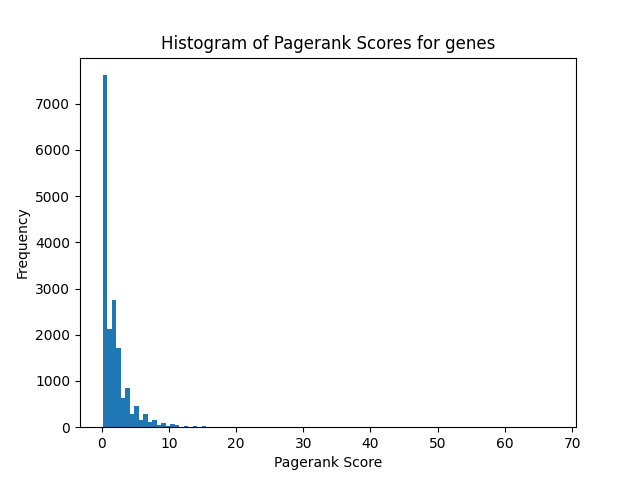
\includegraphics[width=\linewidth]{figures/04_hist_pagerank}
    \endminipage
    \hfill
    \minipage{0.45\textwidth}
      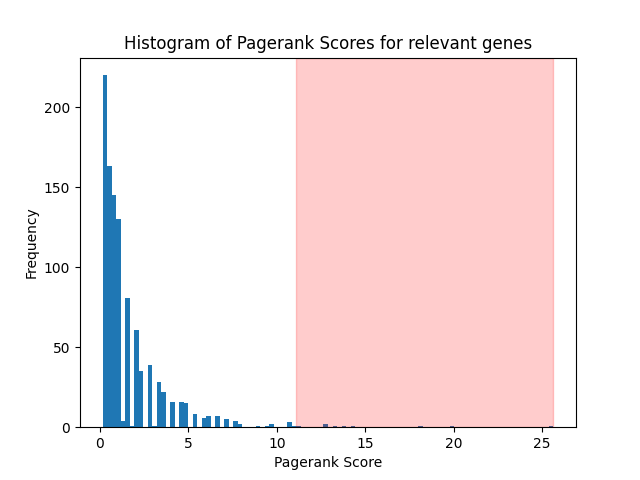
\includegraphics[width=\linewidth]{figures/04_hist_pagerank_relevant}
    \endminipage
    \caption{Comparison of the distribution of Pagerank Scores for all genes and genes with significant change in gene activity
    with highlighted area for the top 10 genes with the highest PageRank scores}
    \label{fig:04_hist_pagerank}
\end{figure}

The $\Delta_{TPM}$ values display a symmetric distribution with a pronounced peak around zero, showing a central tendency near the mean
(see~\cref{fig:04_delta_tpm_relevant}).
The data ranges from -0.709 to 0.423, showing moderate variability, and a normal-like distribution.
The significant change in gene activity is defined as a $\Delta_{TPM}$ value between -0.709 and -0.201 or 0.210 and 0.423.
We observe that 59\% of the relevant genes have an increase in gene activity and 41\% a decrease of activity.\\

\begin{figure}[!h]
    \centering
    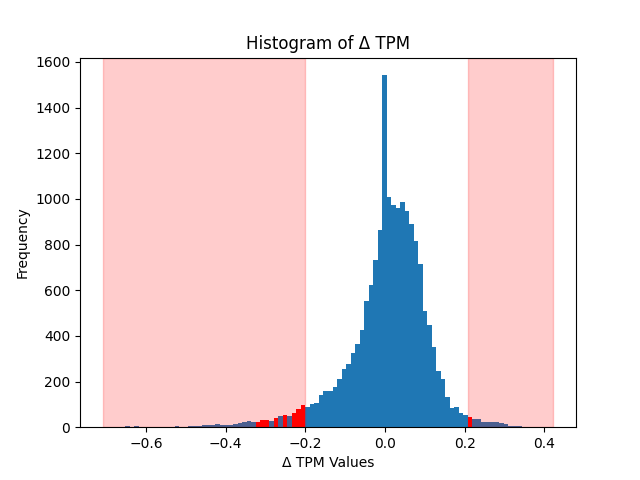
\includegraphics[height=\dfheightdouble]{figures/04_delta_tpm_relevant}
    \caption{Distribution of $\Delta_{TPM}$ values for genes with the area for significant change in gene activity highlighted in red}
    \label{fig:04_delta_tpm_relevant}
\end{figure}


% Presentation of the 10 Genes
To identify the most significant genes, we extracted the \textbf{top 10 genes} with the highest PageRank scores from the list of relevant genes,
as shown in \cref{fig:03_03_df_pagerank_relevant}.
These genes are not only highly connected within the network but also exhibit a substantial change in gene activity.
The PageRank scores are between 25.635 and 11.090,
while the $\Delta_{TPM}$ values span a range from 0.214719 to -0.317776, with only one gene showing a decrease in gene activity.\\


\begin{figure}[!h]
    \centering
    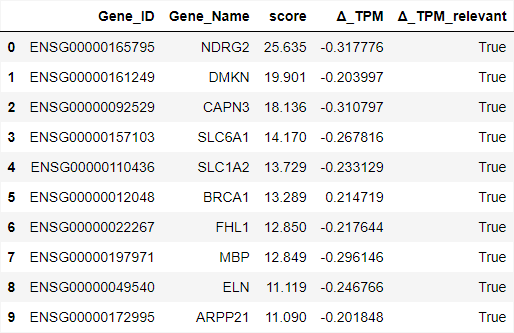
\includegraphics[height=\dfheightdouble]{figures/03_03_df_pagerank_relevant}
    \caption{Top 10 genes with the highest PageRank scores and a significant change in gene activity}
    \label{fig:03_03_df_pagerank_relevant}
\end{figure}

% One Example Gene
As an illustrative example of the structure of the top genes in our network,
we present a gene with high PageRank score and a significant change in gene activity
(see \cref{fig:04_example_gene}).\\

% Cypher: MATCH p = (g:gene {gene_name: 'ELN'})-[r]-(related) RETURN p
\begin{figure}[h]
    \centering
    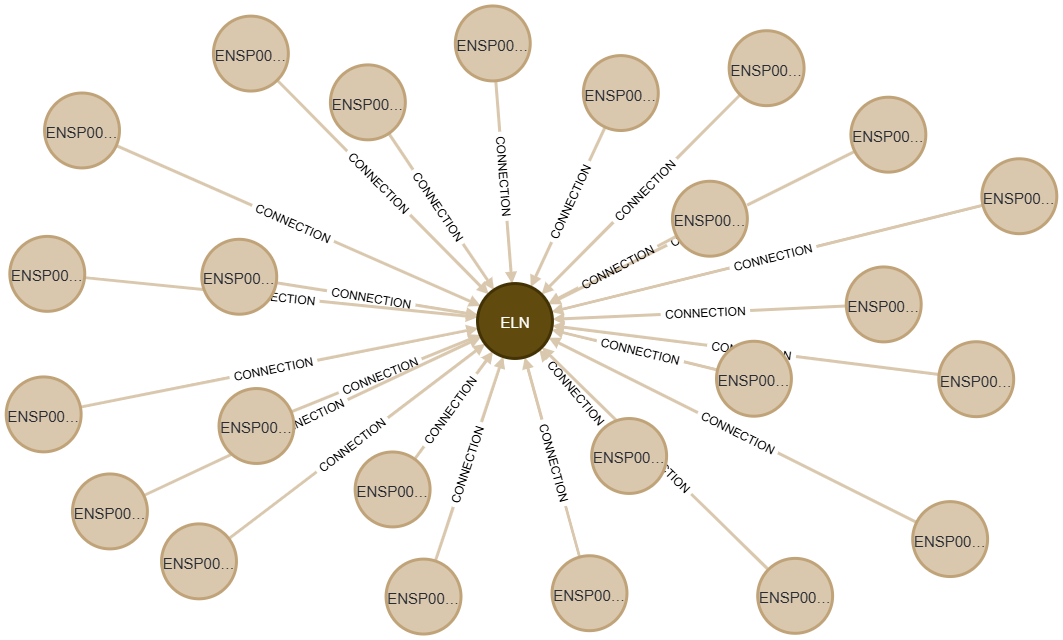
\includegraphics[height=\dfheightdouble]{figures/04_example_gene}
    \caption{An example extract from the graph database for a gene with high PageRank score and significant change in gene activity}
    \label{fig:04_example_gene}
\end{figure}

% Outro
The 10 genes presented here have been identified as key players in the extended PPI network related to lung cancer.
By extracting these top-scoring genes, we not only highlight potential biomarkers but also
shed light on the intricate relationships within this complex biological system.
To further validate these findings, we will conduct a detailed analysis of the current literature and compare our results with existing studies.


\section{Discussion} \label{sec:discussion}
The discussion section that follows delves into the practical implications of our research,
where we examine how the insights gained from analyzing the top 10 genes can be translated into actionable recommendations
for future studies or clinical applications.
We also acknowledge the limitations of our approach and
highlight potential avenues for improving the accuracy and reliability of predictive models in lung cancer diagnosis.

% Alternative
% This chapter delves into the essence of our study,
% where we dissect the results obtained from analyzing the top 10 genes associated with lung cancer biomarkers.
% By examining the relationships between these genes and their potential impact on disease progression,
% we shed light on the complex genetic landscape underlying this malignancy.

% analysius of the results eg Top 10 Pagerank genes
\subsection{Analysis} \label{subsec:analysis}
%general Notes
A first glance at the dataset of all genes reveals the complexity of gene expression in our study.
To establish a foundation for interpreting the results of the top 10 most relevant genes,
we examined the distribution of Pagerank scores and $\Delta\_TPM$ values across the entire dataset

The PageRank scores display an initial peak at approximately 67, which stands out as a significant outlier.
This is followed by a sharp decline to around 40, with subsequent scores showing progressively smaller differences
as they approach the mid-30s range.
Notably, once the scores fall to this level, the gaps between them become considerably narrower.
%TODO This overall distribution suggests a pattern of exponential or logarithmic decay, indicating that the majority of the scores are heavily concentrated towards the higher end.

The data show a symmetric distribution of $\Delta\_TPM$ values, with a pronounced peak around zero, suggesting a central tendency near the mean.
The data ranges approximately from -0.709 to 0.423, indicating moderate variability, and appears to follow a normal-like distribution.
\ref{fig:03_02_delta_tpm}
\newline


% 1 - NDRG2
\textbf{NDRG2} (N-Myc downstream-regulated gene 2) is a tumor suppressor gene that helps control cell growth and
prevents cancer cells from spreading to other parts of the body.
It is particularly important in regulating cells in tissues that are more likely to develop tumors~\cite{Lee2022NDRG2}.

Our analysis reveals that NDRG2 has a PageRank score of 25.635 and is downregulated in lung cancer cells,
with a $\Delta\_TPM$ value of -0.317.
It has the highest delta TPM value among the top 10 genes, indicating a significant decrease in expression levels in lung cancer cells.
\newline

% 2 - DMKN
\textbf{DMKN}, also known as Dermokine, is a gene involved in skin cell function and regulation.
It helps regulate cellular processes in the outer layer of the skin, where it plays a role in maintaining skin health~\cite{Naso2007Deromokine}.

Our analysis reveals that DMKN has a PageRank score of 19.900 and is downregulated in lung cancer cells,
with a $\Delta\_TPM$ value of -0.203.

% 3 - CAPN3
The \textbf{CAPN3} (calpain 3) gene is part of the Calpain system, which includes multiple gene products and proteins.
It is primarily expressed in skeletal muscle cells, where it plays a crucial role in muscle function~\cite{Spinozzi2021Calpain}.

Our analysis reveals that CAPN3 has a PageRank score of 18.136 and is downregulated in lung cancer cells,
with a $\Delta\_TPM$ value of -0.310.
It has the second-highest decrease in expression levels among the top 10 genes.
\newline

% 4 - SLC6A1
\textbf{SLC6A1} is the shorting for the gene solute carrier family 6 member 1,
which encodes a protein that acts as a GABA carrier,
helping to regulate the levels of this neurotransmitter at synapses between neurons~\cite{Chen2020SLC6A1}.

In our analysis the gene has a PageRank score of 14.170 and is downregulated in lung cancer cells,
with a $\Delta\_TPM$ value of -0.267.
\newline

%5 - SLC1A2
The \textbf{SLC1A2}, is another of the family of solute transporter proteins, which is primarily known as glutamat transporter.
It plays a crucial role in regulating glutamate levels in the brain by removing glutamate from synapses.\cite{NCBI2017SLC1A2}

In our analysis the gene has a PageRank score of 13.729 and is downregulated in lung cancer cells,
with a $\Delta\_TPM$ value of -0.233.
\newline

%6 - BRCA1
The \textbf{BRCA1}, Breast Cancer Gene 1, gene is a tumor suppressor gene that produces a protein involved in repairing damaged DNA\@.
It plays a crucial role in maintaining genome stability by facilitating the correct repair of DNA breaks~\cite{NCI2020BRCA1}.

Our analysis reveals that BRCA1 has a PageRank score of 13.288 and is upregulated in lung cancer cells,
with a $\Delta\_TPM$ value of 0.214.
In our Top 10 list it is the only gene that is upregulated in lung cancer cells.
\newline

%7 - FHL1
The \textbf{FHL1} (four and a half LIM domains 1) gene encodes a protein that plays a crucial role in regulating muscle cell differentiation and maturation.
It is primarily expressed in striated muscles but also found in other tissues such as the brain and testis~\cite{Storey2020FHL1}.

Our analysis reveals that FHL1 has a PageRank score of 12.849 and is downregulated in lung cancer cells,
with a $\Delta\_TPM$ value of -0.217.
\newline

%8 - MBP
The \textbf{MBP} (Myelin Basic Protein) gene helps produce proteins that are essential for creating and maintaining the protective covering around nerve fibers,
called myelin.
It also plays a role in helping the body repair damaged nerve coverings and
regulates how immune cells respond to infections or inflammation~\cite{Nye1995MBP}.

Our analysis reveals that MBP has a PageRank score of 12.848 and is downregulated in lung cancer cells,
with a $\Delta\_TPM$ value of -0.296.
\newline

%9 - ELN
The \textbf{ELN} (Elastin) gene encodes for the protein Elastin, which is a key component of connective tissue that provides elasticity and
flexibility to tissues such as skin, lungs, and blood vessels~\cite{Debelle1999ELN}.

Our analysis reveals that ELN has a PageRank score of 11.119 and is downregulated in lung cancer cells,
with a $\Delta\_TPM$ value of -0.246.
\newline

%10 - ARPP21
The \textbf{ARPP21} (cAMP regulated phosphoprotein 21) gene is involved in regulating cellular processes, particularly in brain development and function.
It plays a crucial role in shaping the complexity of neurons during development~\cite{Rehfeld2018ARPP21}.

Our analysis reveals that ARPP21 has a PageRank score of 11.089 and is downregulated in lung cancer cells,
with a $\Delta\_TPM$ value of -0.201.
\newline

% evaluation of my approach and my limitations
\subsection{Study Evaluation} \label{subsec:evaluation}

{\color{lightgray}
* Other datasets could be used like TCGA which is common in cancer research \\
* CMP Dataset matched with ENS ID Names might be wrong - would be better to find a good dataset with ens IDs \\
* Other meseares as TPM or an additional?! \\
* relevant delta TMP might be problmeatic - some genes might be more sensitive to smaller changes \\
* Pagerank might be too focused on first level Proteins \\
    % TODO check how pagerank is implemented
}
% Verallgemeinerung der Daten
% gibt keine Inforamtion über Ethnie
% Especially the focus on the older age range may affect the generalizability of our findings to other populations.


% TODO discussion oder conclusion?
% what can be improved / future work
\subsection{Future Work} \label{subsec:future_work}
{\color{lightgray}
* Pagerank is a good way to find important genes - well established / known / typical research \\
* Clear finding of new genes that may be biomarkers\\
* Analyse the top 10 genes seems to find good results\\

% Future Work
* These should be further investigated in future studies\\
* collective behavior of multiple genes rather than focusing solely on individual genes\\
* Other datasets may be used - especcialy CMP is a bit clupsy with the ENS ID\\
}


\section{Conclusion} \label{sec:conclusion}

% Breif summary of the findings



\section{Notes:}
{\color{lightgray}

preparation of the Datasets for the graph db
* for every dataset we need the format genes as rows and at least the ENS ID and a mean tpm for every gene row
    * GTEX (Genotype-Tissue Expression) - healthy tissues
        * downloaded bulk-tissue-expression file (... more about the data)
        * format was: Gene / ENS ID as rows and tissues as columns - tpm value for every gene in every tissue
        * melted down to genes as rows and tissue and tpm value as columns
        * grouped by tissues to get a single tpm value for every gene (eigentlich sum and count to get mean)
    → 56.156 human genes with mean values for healthy tpm

    * CMP (Cell Model Passport) - cancerous tissues
        * downloaded all RNA-Seq processed data - which contain data from Sanger Institute and from Broad Institute
        * format was: genes with CMP IDs as rows and tpms, tissues (called model), ... per column
        * separate file loaded with model annotation to get a list of all models (tissues) that have lung cancer as cancer type
        * filtered the data to get only the lung cancer models
        * grouped all models (tissues) to get a mean tpm value for every gene
        * needed to add ENS ID to the genes for further processing
        * separate ensemble file downloaded from biomart (https://www.ensembl.org/biomart/martview/)
        * contains Gene stable ID and gene symbol (name)
        * idea is to add the Gene stable ID by merging both tables by the gene name
        * daher gehen wir davon aus, dass jeder gen name eindeutig ist
        * war es nicht - 10.605/48.311 rows in the ensemble file had a not unique gene name
        * rows with names that are not unique were removed
        * merging the ensemble file with the CMP data to get the ENS ID for every gene
        * 3.760 / 37.262 genes had no ENS ID → missing IDs could be added by synonymes maybe because of duplicate removement
        * these genes are removed
    → 33.502 human genes with mean values tpm for lung cancer

Datasets to nodes and edges
    * genes as nodes
        * eigenschaft: name, gene stable id, norm healyth tpm, norm cancerous tpm, delta tpm, z score, delta tpm relevant
        * merging the GTEx (healthy) and CMP (cancerous) data to get a list of all genes that are in both datasets
        * filtering for genes that have a gene-protein connection
        * normalizing the TPM Values with log scaling
        * calculate a delta TPM value for every gene as the difference between the mean tpm value in the healthy and the cancerous dataset
        * NOT THE ABSOLUTE
        * to find out which genes have a relevant change in the healthy and cancerous tpm value we calculate the z score for the delta tpm values for every gene
        * z score is calculated as the difference between the delta tpm value and the mean delta tpm value divided by the standard deviation of the delta tpm values
        * z score is a measure of how many standard deviations an element is from the mean
        * XXX genes with a z score of 1,96 or higher are considered as delta tpm relevant (p Wert damit 0,05 and Konfidenzniveau 95%)
    → 17.626 gene Nodes

    * protein-gene connection as edges
        * eigenschaft: gene stable id, protein stable id
        * proteins are needed as a second node type to get a connection between the genes.
        * downloaded protein file from biomart with gene stable ID and protein stable ID
        * filtered for those gene stable IDs that are in the gene node list.
        * we only have those proteins that have a connection (was sagt die tabelle genau aus?)
    → 101.731 protein gene edges (means: every protein is connected to exactly one gene, but every gene can have multiple proteins)

    * proteins as nodes
        * eigenschaft: protein stable id
        * use the protein gene table as base
        * only use the column with the protein stable ID
    → 101.731 protein Nodes

    * protein protein connection as edges
        * eigenschaft: protein stable id 1, protein stable id 2
        * downloaded protein protein interaction file from STRING database
        * filtered for those protein stable IDs that are in the protein node list
    → 11.247.242 protein protein edges
    (not every protein is connected to another one → but since every gene could have multiple proteins, the connected gene may have a connection to another protein)
    TODO: are those genes that are not connected to another gene relevant for the analysis?

Graph database
    * Neo4J
    * gene nodes query:
    * protein nodes query:
    * gene protein edges query:
    * protein protein edges query:

}


\newpage
\bibliographystyle{plain} % We choose the "plain" reference style
\bibliography{refs} % Entries are in the refs.bib file

\end{document}